\documentclass[12pt]{article}

\usepackage[a4paper, margin=0.5in]{geometry}
\usepackage{anyfontsize}
\usepackage{xcolor}
\usepackage{graphicx}
\usepackage{setspace}
\usepackage{hyperref}
\usepackage[backend=biber]{biblatex}
\usepackage{float}
\usepackage{svg}
\usepackage{xepersian}
\usepackage{amssymb}
\usepackage{amsmath}
\usepackage{enumitem}
\usepackage{caption}
\usepackage{bigints}
\hypersetup{colorlinks,urlcolor=blue}
%\settextfont[Scale=1.1]{Far.Mitra}

\settextfont[Scale=1.0, Size=14pt]{B Nazanin}
\defpersianfont\persiantitlefont[Scale=1.0, Size=18pt]{B Titr}
\setlatintextfont[Scale=1.0, Size=12pt]{Times New Roman}
\deflatinfont\englishtitlefont[Scale=1.0, Size=16pt]{Times New Roman Bold}
\definecolor{mediumpersianblue}{rgb}{0.0, 0.4, 0.65}
\usepackage[backend=biber]{biblatex}
\addbibresource{references.bib}


\def\labelitemi{$\diamond$}
\def\labelitemii{$\ast$}


\begin{document}
	\linespread{3}
	\setstretch{1.5}
	

	\begin{minipage}[t]{0.7\textwidth}
		
		{\huge\textcolor{mediumpersianblue!70!black}{\title\textbf{{ رباتیک}}}}\\[4pt]
		
	\end{minipage}
	\hfil
	\begin{minipage}[t]{0.15\textwidth}
		\centering
		
\includegraphics[width=0.9\linewidth]{pics/logo.png}\\[6pt]
		{\small پاییز ۱۴۰۴}
	\end{minipage}
	
	
	
	{
		
		\Large{پروژه اول}
		
		\large مرتضی ملکی‌نژاد شوشتری - ۸۱۰۱۰۴۲۵۶ 
		
		
	}
	
	\vspace{1.2cm}
	
	
	
	\vspace{0.3cm}
	\hrule 
	\vspace{0.6cm}
	\lr{\section{Forward and Inverse Kinematics}}
	\subsection{جدول \lr{DH} ربات}
	{
		\centering
		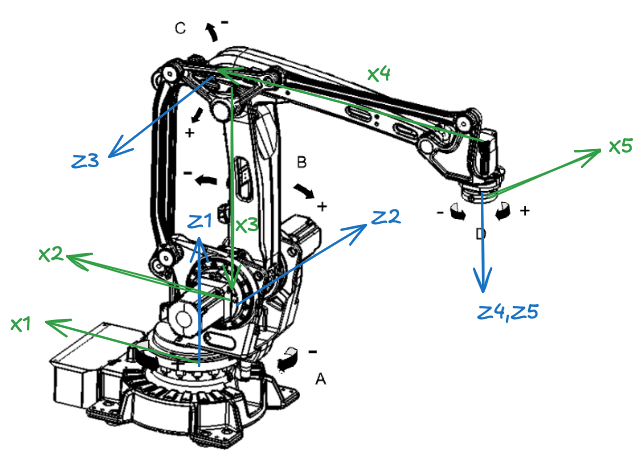
\includegraphics[width=0.8\textwidth]{pics/dh_axis.png}
		\captionof{figure}{محورهای \lr{DH} ربات}
	}
	{
		\centering
		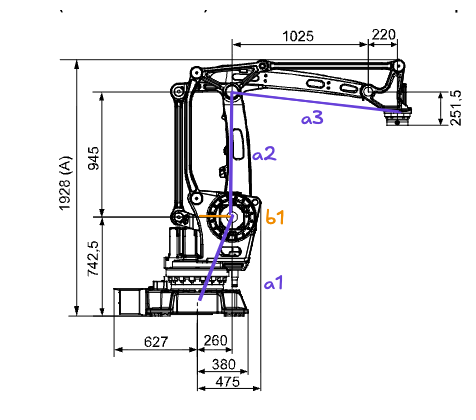
\includegraphics[width=0.8\textwidth]{pics/dh_params.png}
		\captionof{figure}{پارامترهای انتقالی \lr{DH} ربات}
	}
            \begin{table}[ht]
	\centering
\caption{جدول پارامترهای \lr{DH} ربات (با دقت دو رقم اعشار)}
	\label{tab:dh-table}
	\begin{latin}
		
		\begin{tabular}{c | ccc c}
			number & $a$ & $b$ & $\alpha$ & $\theta$ \\
			\hline
			1 & 786.71 & 260 & $\cfrac{\pi}{2} $ & $\theta_1$ \\
			2 & 945  & 0 & $\pi$ & $\theta_2 - \cfrac{\pi}{2}$ \\
			3 & 1270.15 & 251.5 & $\cfrac{3\pi}{2}$ &  $\theta_3 - \cfrac{\pi}{2}$ \\
			4 & 0 & 0 & 0 & $\theta_4 + \cfrac{\pi}{2}$ \\
		\end{tabular}
	\end{latin}
\end{table}
\subsection{محاسبه بردارهای انتقال و ماتریس‌های دوران}
\begin{latin}

$
	Q_1 = \begin{bmatrix}
		\cos(\theta_1) & 0 & \sin(\theta_1) \\
		\sin(\theta_1) & 0 & -\cos(\theta_1) \\
		0 & 1 & 0
	\end{bmatrix}
	\mathbf{a}_1 = \begin{bmatrix}
		786.71\cos(\theta_1) \\
		786.71\sin(\theta_1) \\
		260
	\end{bmatrix} 
	 \\[2em]
	Q_2 = \begin{bmatrix}
		\sin(\theta_2) & -\cos(\theta_2) & 0 \\
		-\cos(\theta_2) & -\sin(\theta_2) & 0 \\
		0 & 0 & -1
	\end{bmatrix}
	\mathbf{a}_2 = \begin{bmatrix}
		945\sin(\theta_2) \\
		-945\cos(\theta_2) \\
		0
	\end{bmatrix}
	 \\[2em]
	Q_3 = \begin{bmatrix}
		\sin(\theta_3) & 0 & \cos(\theta_3) \\
		-\cos(\theta_3) & 0 & \sin(\theta_3) \\
		0 & -1 & 0
	\end{bmatrix}
	\mathbf{a}_3 = \begin{bmatrix}
		1270.15\sin(\theta_3) \\
		-1270.15\cos(\theta_3) \\
		251.50
	\end{bmatrix}
	 \\[2em]
	Q_4 = \begin{bmatrix}
		-\sin(\theta_4) & -\cos(\theta_4) & 0 \\
		\cos(\theta_4) & -\sin(\theta_4) & 0 \\
		0 & 0 & 1
	\end{bmatrix}
	\mathbf{a}_4 = \begin{bmatrix}
		0 \\
		0 \\
		0
	\end{bmatrix}
$
\end{latin}
\subsection{معادلات \lr{Forward} ربات}
{
	\footnotesize
\begin{latin}
	$$
	Q = 
	\begin{bmatrix}
		\sin(\theta_1)\cos(\theta_4) - \sin(\theta_4)\cos(\theta_1)\cos(\theta_2-\theta_3)
		& -\sin(\theta_1)\sin(\theta_4) - \cos(\theta_1)\cos(\theta_4)\cos(\theta_2-\theta_3)
		& \sin(\theta_2-\theta_3)\cos(\theta_1)
		\\[6pt]
		-\sin(\theta_1)\sin(\theta_4)\cos(\theta_2-\theta_3) - \cos(\theta_1)\cos(\theta_4)
		& -\sin(\theta_1)\cos(\theta_4)\cos(\theta_2-\theta_3) + \sin(\theta_4)\cos(\theta_1)
		& \sin(\theta_1)\sin(\theta_2-\theta_3)
		\\[6pt]
		-\sin(\theta_4)\sin(\theta_2-\theta_3)
		& -\cos(\theta_4)\sin(\theta_2-\theta_3)
		& -\cos(\theta_2-\theta_3)
	\end{bmatrix}
	\\	
	$$
\end{latin}
}
\subsection{مسیر حرکت}
با رسم مسیر حرکت (با استفاده از ماتریس‌های \lr{T}) مي‌توان مختصات مفاصل را بدست آورد. :
~\\
{
\centering
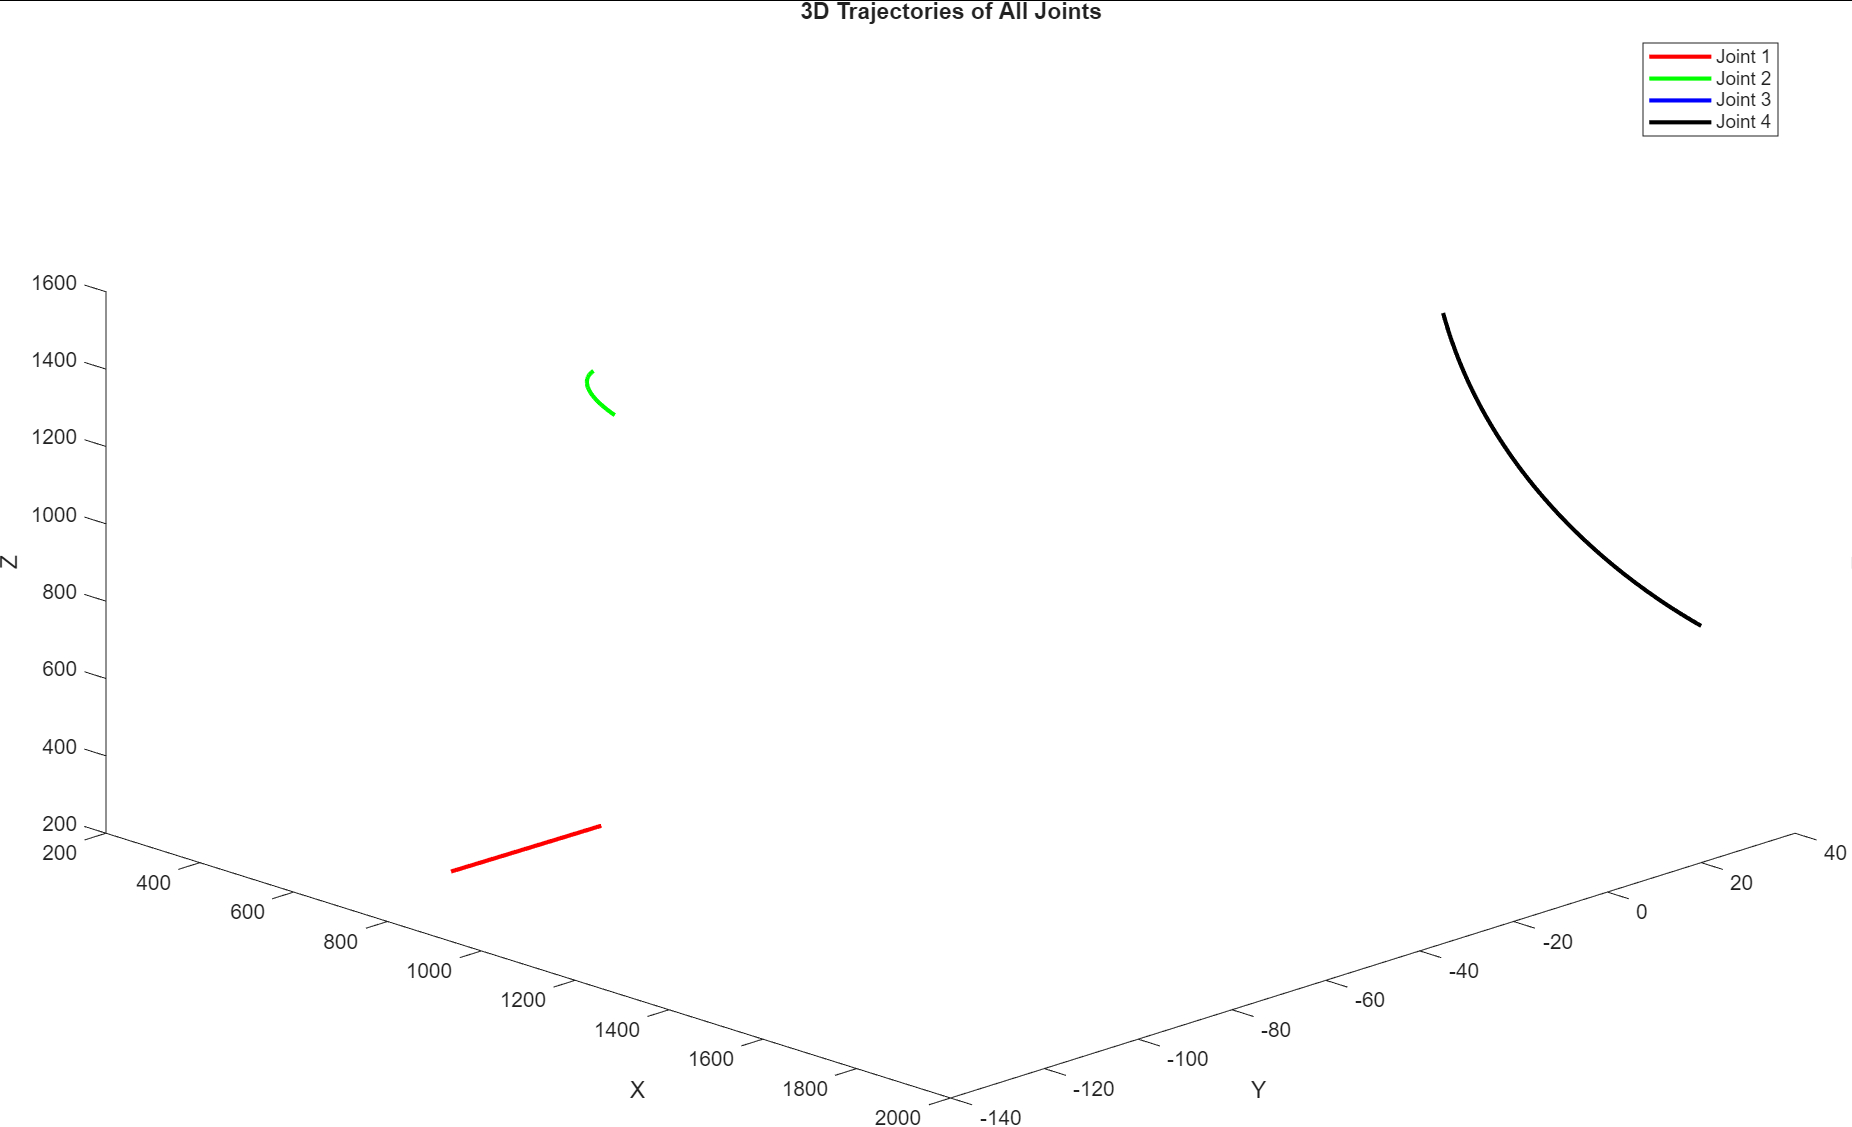
\includegraphics[width=0.8\textwidth]{pics/q1_1.jpeg}
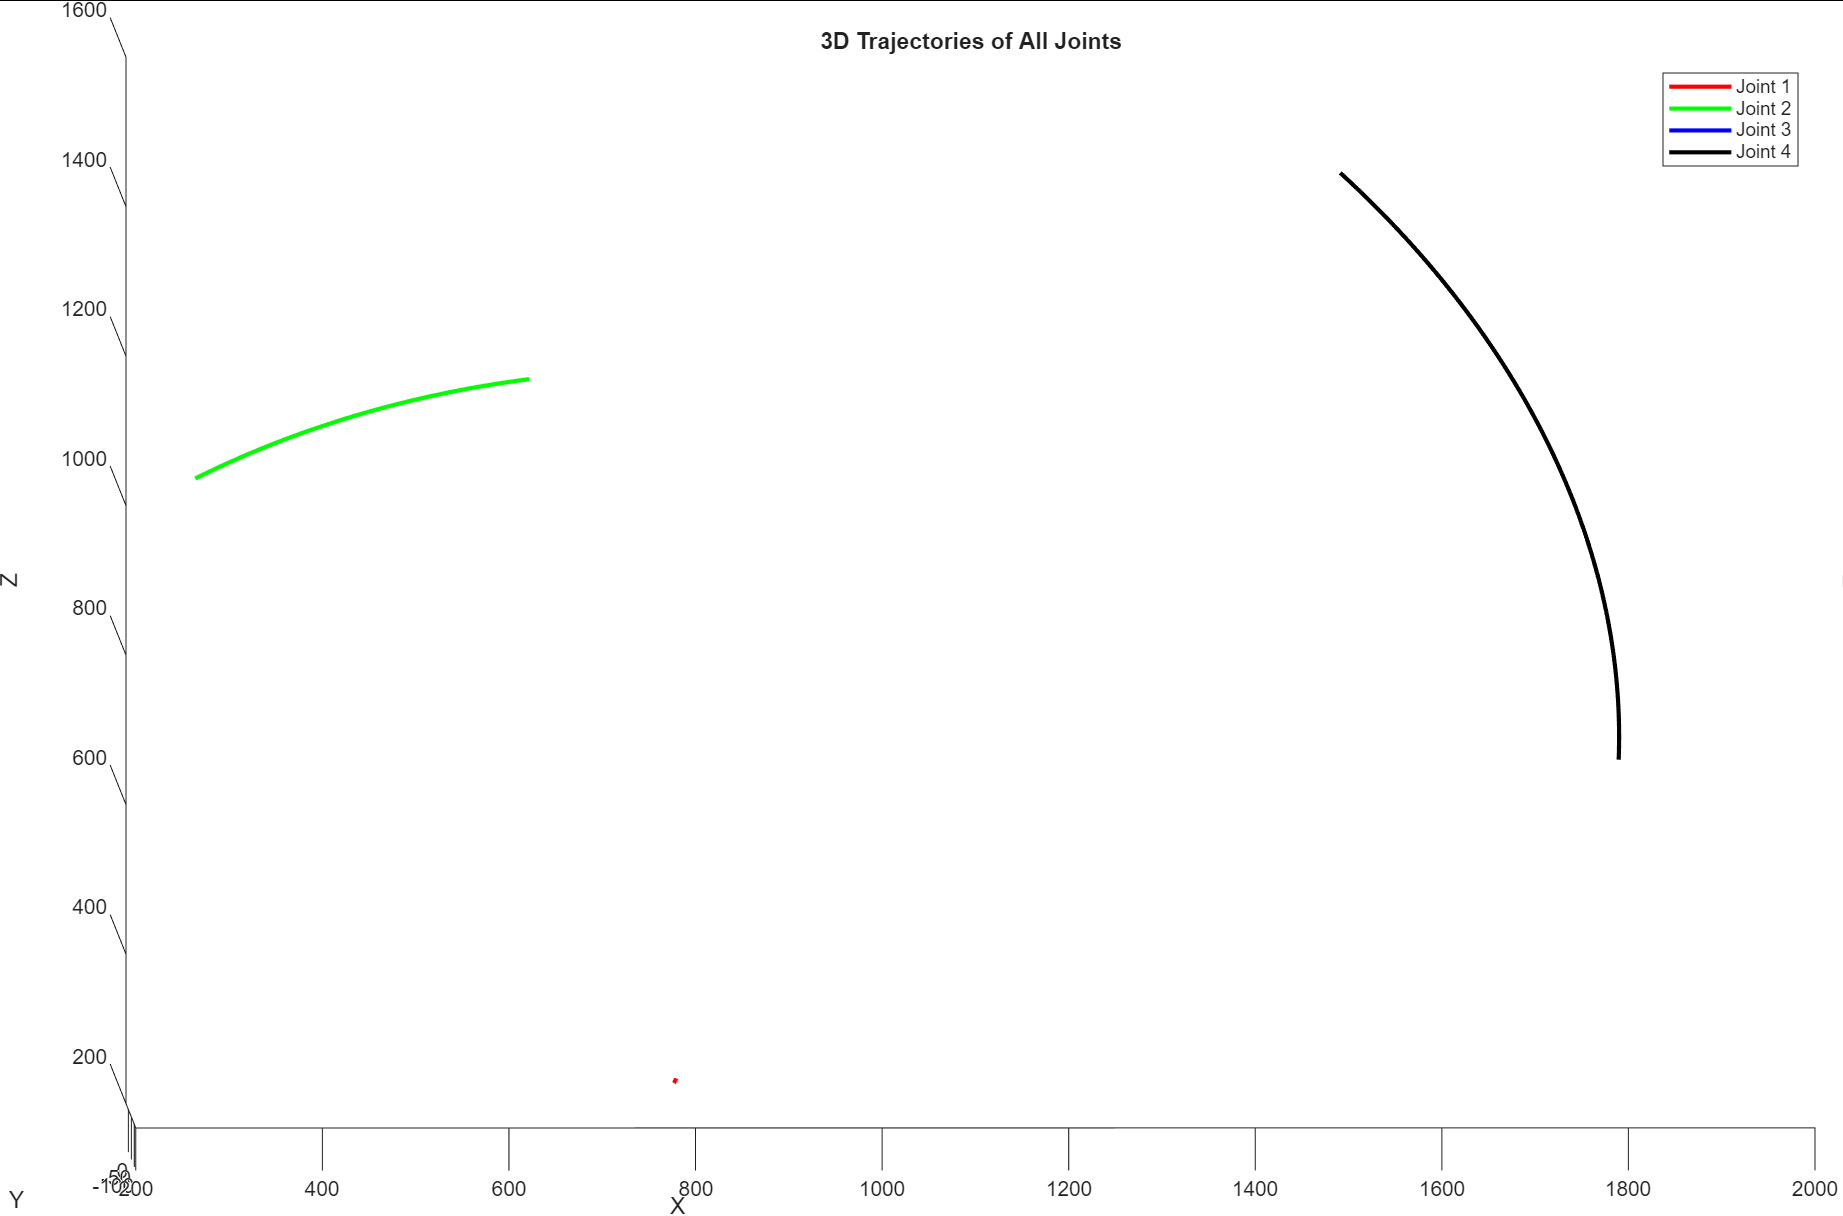
\includegraphics[width=0.8\textwidth]{pics/q1_2.jpeg}
\captionof{figure}{مسیر حرکت مفاصل از مبدا به مقصد با فرض خطی. همانطور که در نمای \\lr{XZ} مشخص است، می‌توان  به طور شهودی دید این ربات با ربات سوال یکی است.. در شکل ۳ و ۴ روی هم هستند.}
}
\section{برنامه ریزی مسیر}
کد این قسمت در فایل 
\lr{q2.m}
آمده است. چون عملا خود سوال دستورالعمل بخش به بخش پیاده‌سازی است، کد توضیح داده نشده.
{
	\centering
	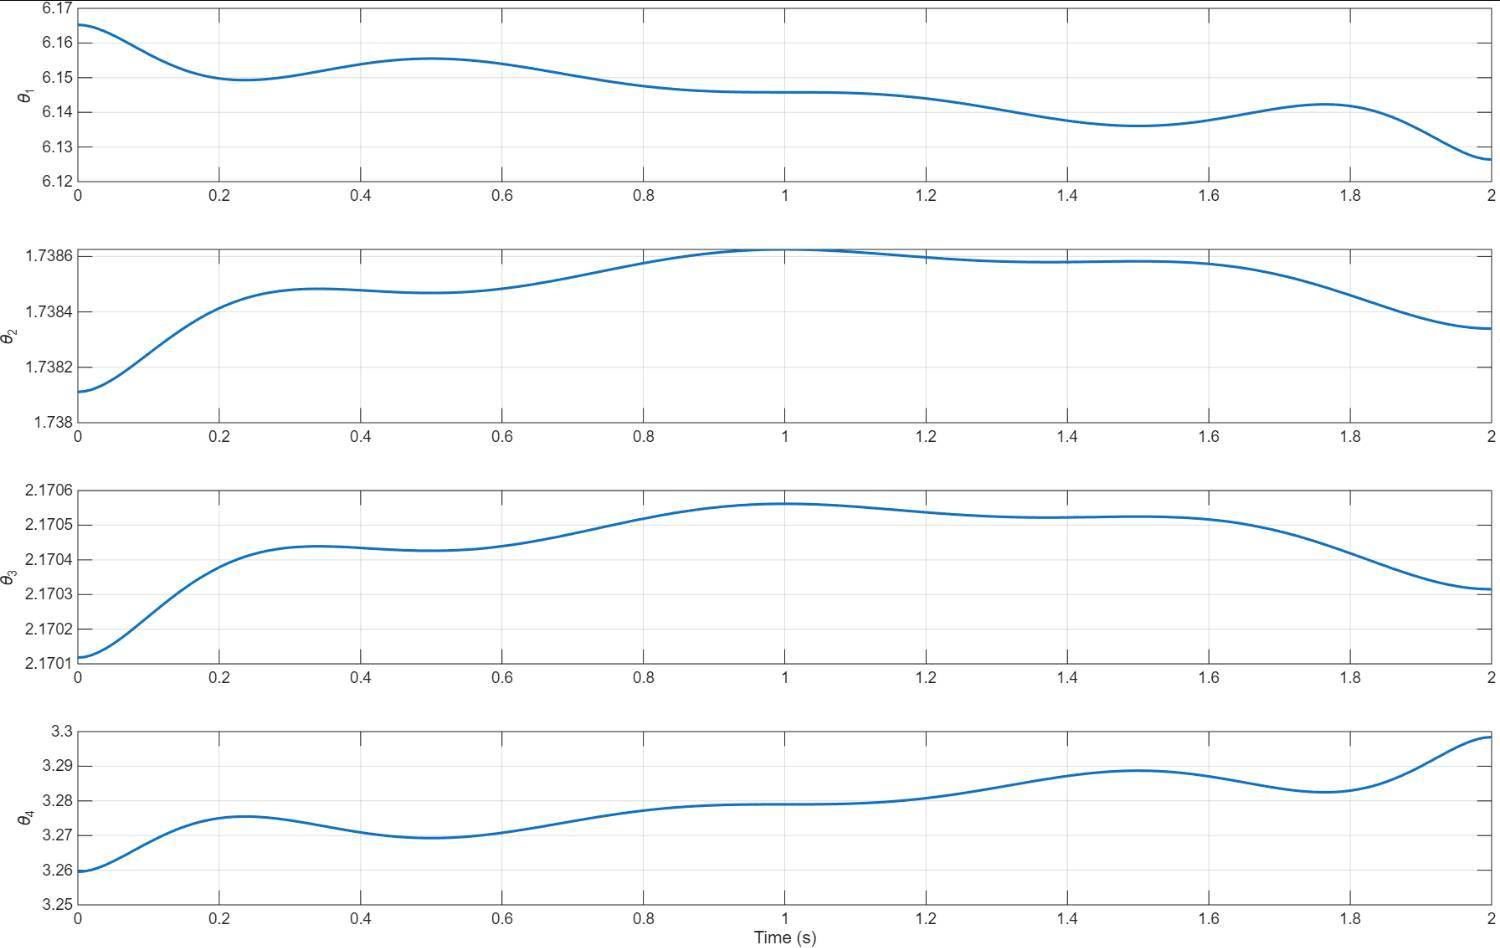
\includegraphics[width=0.8\textwidth]{pics/q2_1.jpeg}
	\captionof{figure}{مقادیر $\theta$ در گذر زمان.}
}
{
	\centering
	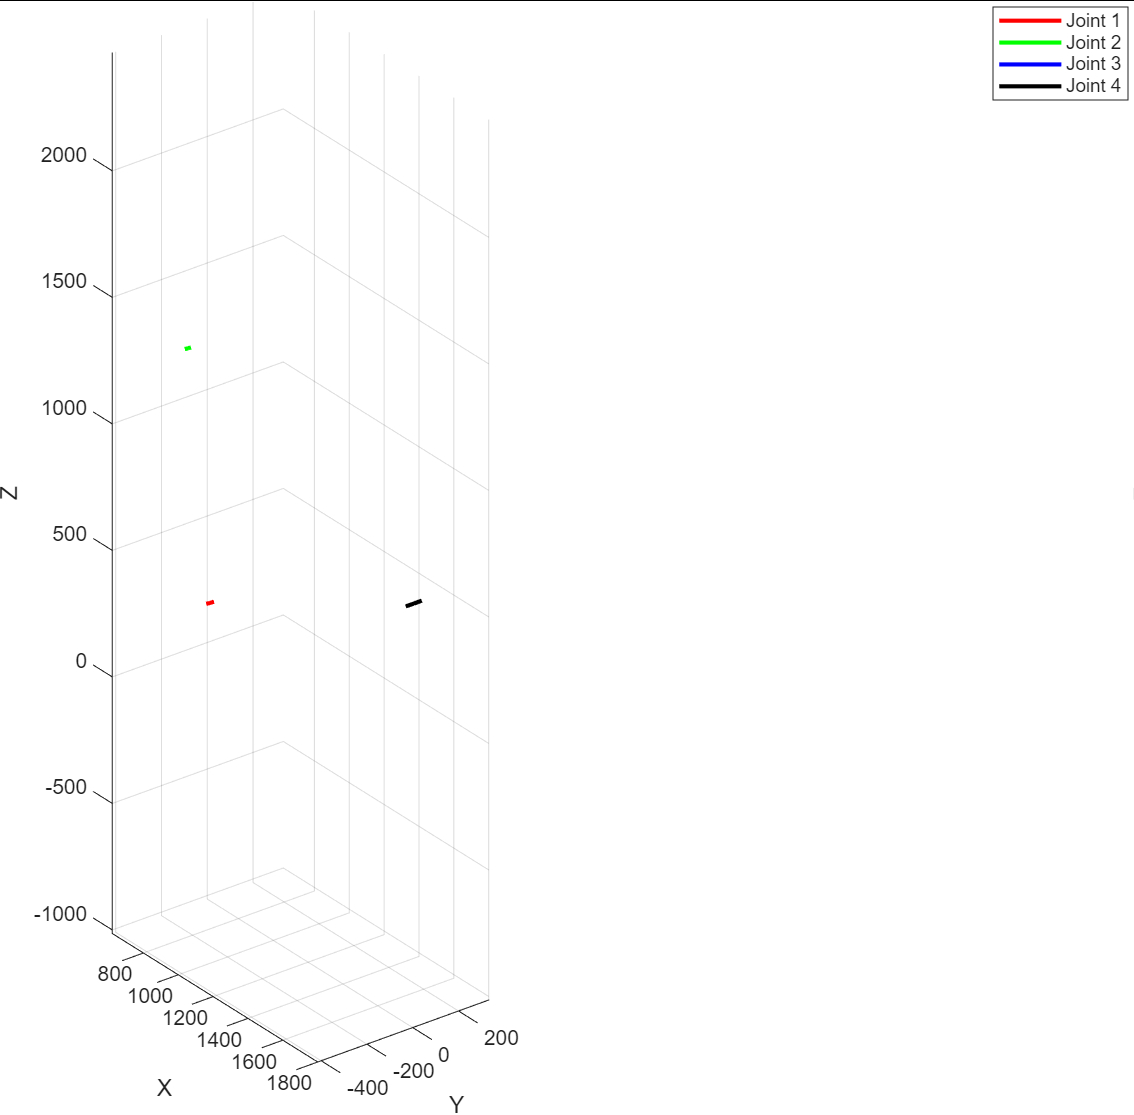
\includegraphics[width=0.8\textwidth]{pics/q2_2.jpeg}
	\captionof{figure}{همانطور که انتظار می‌رفت تنها تغییر مجری نهایی در راستای \lr{y} می‌باشد.}
}
اگر مفاصل در راستای دیگری نیز حرکت داشتند، به این معنی است که ربات به نقط تکین نزدیک شده است زیرا در عمل چندین مفصل دارند حرکت همدیگر را خنثی می‌کنند. در اینصورت یکی از راه‌ها حذف یک درجه آزادی از ربات است (مثلا مقدار $\phi$ را آزاد گذاشت.) یا برای مثال می‌توان 
\lr{Condition number}
ماتریس ژاکوبین را در برنامه‌ریزی مسیر دخیل کرد تا ماتریس از نقاط تکین دوری کند.
\end{document}